\section{Compute configuration}
\label{system-architecture-and-implementation:compute-configuration}
This section specifies the engines that query the representations the data layer fixes, the levels of the configuration factor defined in Section~\ref{research-design-and-methodology:overview-and-experimental-design:factors-and-levels}. Three engines carry their own compute configuration and are described here: DuckDB running in-process over GeoParquet, PostGIS on a managed PostgreSQL server, and Apache Sedona on a transient Databricks cluster. The local GeoPandas baseline reads the Shapefile bundle of Section~\ref{system-architecture-and-implementation:data-layer} with no further configuration and is not revisited. Each engine otherwise keeps its published defaults and departs from them only where a measurement concern requires it, so that incidental tuning cannot account for an observed difference. The two single-node engines come first, DuckDB then PostGIS, followed by the distributed Sedona configuration.

\subsection{DuckDB}
\label{system-architecture-and-implementation:compute-configuration:duckdb}

DuckDB reads GeoParquet directly from object storage, with no server process standing between the engine and the data. Every benchmark runs the pinned version \texttt{1.4.0} in-process inside the query \acrshort{aci} container. At connection time the engine installs and loads two extensions: \texttt{spatial}, for the \acrshort{ogc} Simple Features geometry type and the \texttt{ST\_} function library, and \texttt{azure}, for native access to \acrshort{adls}. Authentication uses a DuckDB secret created with \texttt{PROVIDER config} and bound to the storage account name, so \texttt{az://} paths resolve without a connection string\footnote{A connection string is the single text value encoding the server address, database, and credentials a client uses to open a connection.} in the query text. On Linux, \texttt{azure\_transport\_option\_type} is set to \texttt{curl} to avoid the problems DuckDB's default Azure HTTP client exhibits in the container environment.

Each query reads the buildings dataset through \texttt{read\_parquet} over an \texttt{az://} path, so DuckDB applies to remote Parquet the predicate and projection pushdown described in Section~\ref{background:spatial-data-formats-and-storage-models:full-database-engines:duckdb-with-the-spatial-extension}. The pushdown fetches only the row groups and columns a query references, realizing the range-request access pattern of Section~\ref{background:spatial-data-formats-and-storage-models:summary}. The three \acrshort{rq}1 query patterns follow the workload definitions in Section~\ref{research-design-and-methodology:workloads:workload-definitions}, expressed in DuckDB's \acrshort{sql} dialect. The point-in-polygon lookup evaluates \texttt{ST\_Contains} against a fixed probe point. The $k$-nearest-neighbor search orders the buildings by \texttt{ST\_Distance} to a fixed reference point and takes the first $k = \num{10}$; DuckDB has no native nearest-neighbor index, so the query resolves as a full scan followed by a sort. The bounding-box filter pairs an \texttt{ST\_Intersects} test against a fixed rectangular window with an area predicate, \texttt{ST\_Area} of the geometry reprojected to EPSG:25832 exceeding \SI{10}{\meter\squared}.

\subsection{PostGIS}
\label{system-architecture-and-implementation:compute-configuration:postgis}

PostGIS fills the traditional single-node cell, reading the buildings dataset from server-managed tables rather than directly from object storage. The engine is PostgreSQL~17 with the PostGIS~3.5.2 extension, running on the Azure Database for PostgreSQL Flexible Server whose \acrshort{sku} and sizing are fixed in Section~\ref{system-architecture-and-implementation:infrastructure:compute-platforms}. One instance backs every PostGIS workload across all size tiers, so all PostGIS results share a single server configuration. Each query container reaches the server through a SQLAlchemy engine over the \texttt{psycopg2} driver\footnote{SQLAlchemy is a Python database-access toolkit; \texttt{psycopg2} is the driver through which it communicates with PostgreSQL.}, and on creation that engine issues \texttt{CREATE EXTENSION IF NOT EXISTS postgis}, matching the \texttt{azure.extensions} allowlist of Section~\ref{system-architecture-and-implementation:data-layer:postgis-on-azure-postgresql}. The size-tier tables and their \acrshort{gist} spatial indexes are built once during setup, as detailed in that section, so every timed run reads from a server already in its final state. Each timed iteration opens its connection through \texttt{connect()} inside the timed function, never reusing a handle from before the measured window.

The three \acrshort{rq}1 query patterns reuse the DuckDB formulations, expressed in PostGIS's \acrshort{sql} dialect and following the workload definitions in Section~\ref{research-design-and-methodology:workloads:workload-definitions}. The point-in-polygon lookup evaluates \texttt{ST\_Contains} against the same fixed probe point. The k-nearest-neighbor search orders the buildings by the \texttt{<->} operator relative to a fixed reference point and takes the first $k = \num{10}$, which resolves as a \acrshort{gist} index-ordered scan rather than the DuckDB scan-and-sort. The \texttt{<->} operator ranks candidates by bounding-box distance, an approximation that is negligible for the small building polygons used here. The bounding-box filter applies both an \texttt{ST\_Intersects} test against a fixed rectangular window and an area predicate, \texttt{ST\_Area} of the geometry reprojected to EPSG:25832 exceeding \SI{10}{\meter\squared}.

\subsection{Apache Sedona on Databricks}
\label{system-architecture-and-implementation:compute-configuration:apache-sedona-on-databricks}

The distributed configuration is a set of pinned library versions running on a transient Azure Databricks cluster. Apache Sedona 1.7.1 is installed as the shaded Maven artifact\footnote{Maven is the Java build and dependency-management system; a \enquote{shaded} artifact bundles a library's dependencies under renamed packages so they cannot clash with versions already on the class path.} \texttt{org.apache.\allowbreak sedona:sedona-spark-shaded-3.5\_2.12:1.7.1}, together with the \acrshort{pypi}\footnote{PyPI is the Python Package Index, the default repository from which \texttt{pip} installs Python packages.} packages \texttt{apache-sedona==1.7.1} and \texttt{geopandas==0.14.4}, on Databricks Runtime 15.4 \acrshort{lts} (Spark version \texttt{15.4.x-scala2.12}). Every node, driver and worker alike, is a \texttt{Standard\_D4s\_v3} virtual machine. The cluster is provisioned once and its libraries requested, and the run blocks until the cluster reports \texttt{RUNNING} and every library reports \texttt{INSTALLED}, after which the benchmark notebook\footnote{A notebook is an executable document that interleaves code cells with their output; Databricks runs the benchmark as one such document.} is uploaded to the workspace. The single warmup iteration and the three timed iterations then submit against this one warm cluster, mirroring the provision-once discipline established in Section~\ref{research-design-and-methodology:overview-and-experimental-design:replication-and-randomization}. A \texttt{finally} block terminates the cluster even when an iteration raises. The cluster is created in \texttt{LEGACY\_SINGLE\_USER} mode with \texttt{single\_user\_name} resolved from the \acrshort{scim} \texttt{/Me} endpoint\footnote{SCIM abbreviates System for Cross-domain Identity Management, a standard protocol for exchanging user-identity data; its \texttt{/Me} endpoint returns the calling user's own identity.}, which the workspace's Unity Catalog\footnote{Unity Catalog is Databricks's centralized governance layer for access control over data and compute across a workspace.} enforcement requires before it will accept a cluster-creation request.

Several Spark settings are fixed at cluster creation so that the join executes under the measured plan rather than one the platform substitutes. Photon, the vectorized execution engine Databricks layers over Spark, is disabled (\texttt{spark.databricks.photon.enabled=false}): it bypasses the Catalyst strategies that Sedona registers, which would force the spatial join into a BroadcastNestedLoopJoin, a brute-force evaluation that pairs every record on one side with every record on the other. \acrfull{aqe} is disabled (\texttt{spark.sql.adaptive.enabled=false}) and automatic broadcasting is switched off (\texttt{spark.sql.autoBroadcastJoinThreshold=-1}), because \acrshort{aqe} can rewrite a Sedona spatial-join plan at execution time and Spark's broadcast heuristic can otherwise pre-empt the partitioned strategy before it runs \parencite{spark2024_sql_performance_tuning}. The cluster uses Kryo serialization\footnote{Kryo is a fast Java object-serialization library that Spark can use in place of default Java serialization to encode objects for shuffle and caching.} (\texttt{spark.serializer} set to \texttt{org.apache.spark.serializer.KryoSerializer}). The driver allocation is fixed at \texttt{9g} of memory with \texttt{1g} of overhead and a \texttt{4g} cap on the collected result.

The broadcast and partitioned join strategies distinguished in Section~\ref{background:distributed-spatial-processing:distributed-spatial-operations} are encoded as two notebook variants. The broadcast variant wraps the smaller municipalities input in Spark's \texttt{broadcast()} hint, so Sedona plans the join as a BroadcastIndexJoin\footnote{BroadcastIndexJoin is the Spark physical-plan operator that realizes the broadcast strategy, joining each partition of the larger input against the broadcast copy of the smaller one.} and ships the municipality boundaries to every executor. The partitioned variant instead sets \texttt{sedona.global.index=true}, \texttt{sedona.join.gridtype=\allowbreak kdbtree}, and \texttt{sedona.join.indexbuildside=right}, so the join executes as a RangeJoin\footnote{RangeJoin is the Spark physical-plan operator that realizes the partitioned strategy, evaluating the spatial predicate within each pair of spatially co-partitioned cells.} over a KDB-Tree partitioning with the per-partition index built on the buildings side \parencite{sedona2024_spatial_sql_application}. Both variants repartition the buildings to the cluster's \texttt{defaultParallelism}, the worker count multiplied by the four cores of each \texttt{Standard\_D4s\_v3} node, so that work spreads across every executor rather than concentrating on a straggler. Figure~\ref{fig:sedona-join-plan-control} shows how the shared guardrails and the per-variant settings steer the join to each physical plan. A third variant that left plan selection to Spark's cost-based optimizer was implemented as an untuned baseline but dropped from the study, because its iterations consistently timed out or failed at this workload's scale, which made reliable measurement infeasible within the run-time budget.

\begin{figure}[H]
    \centering
    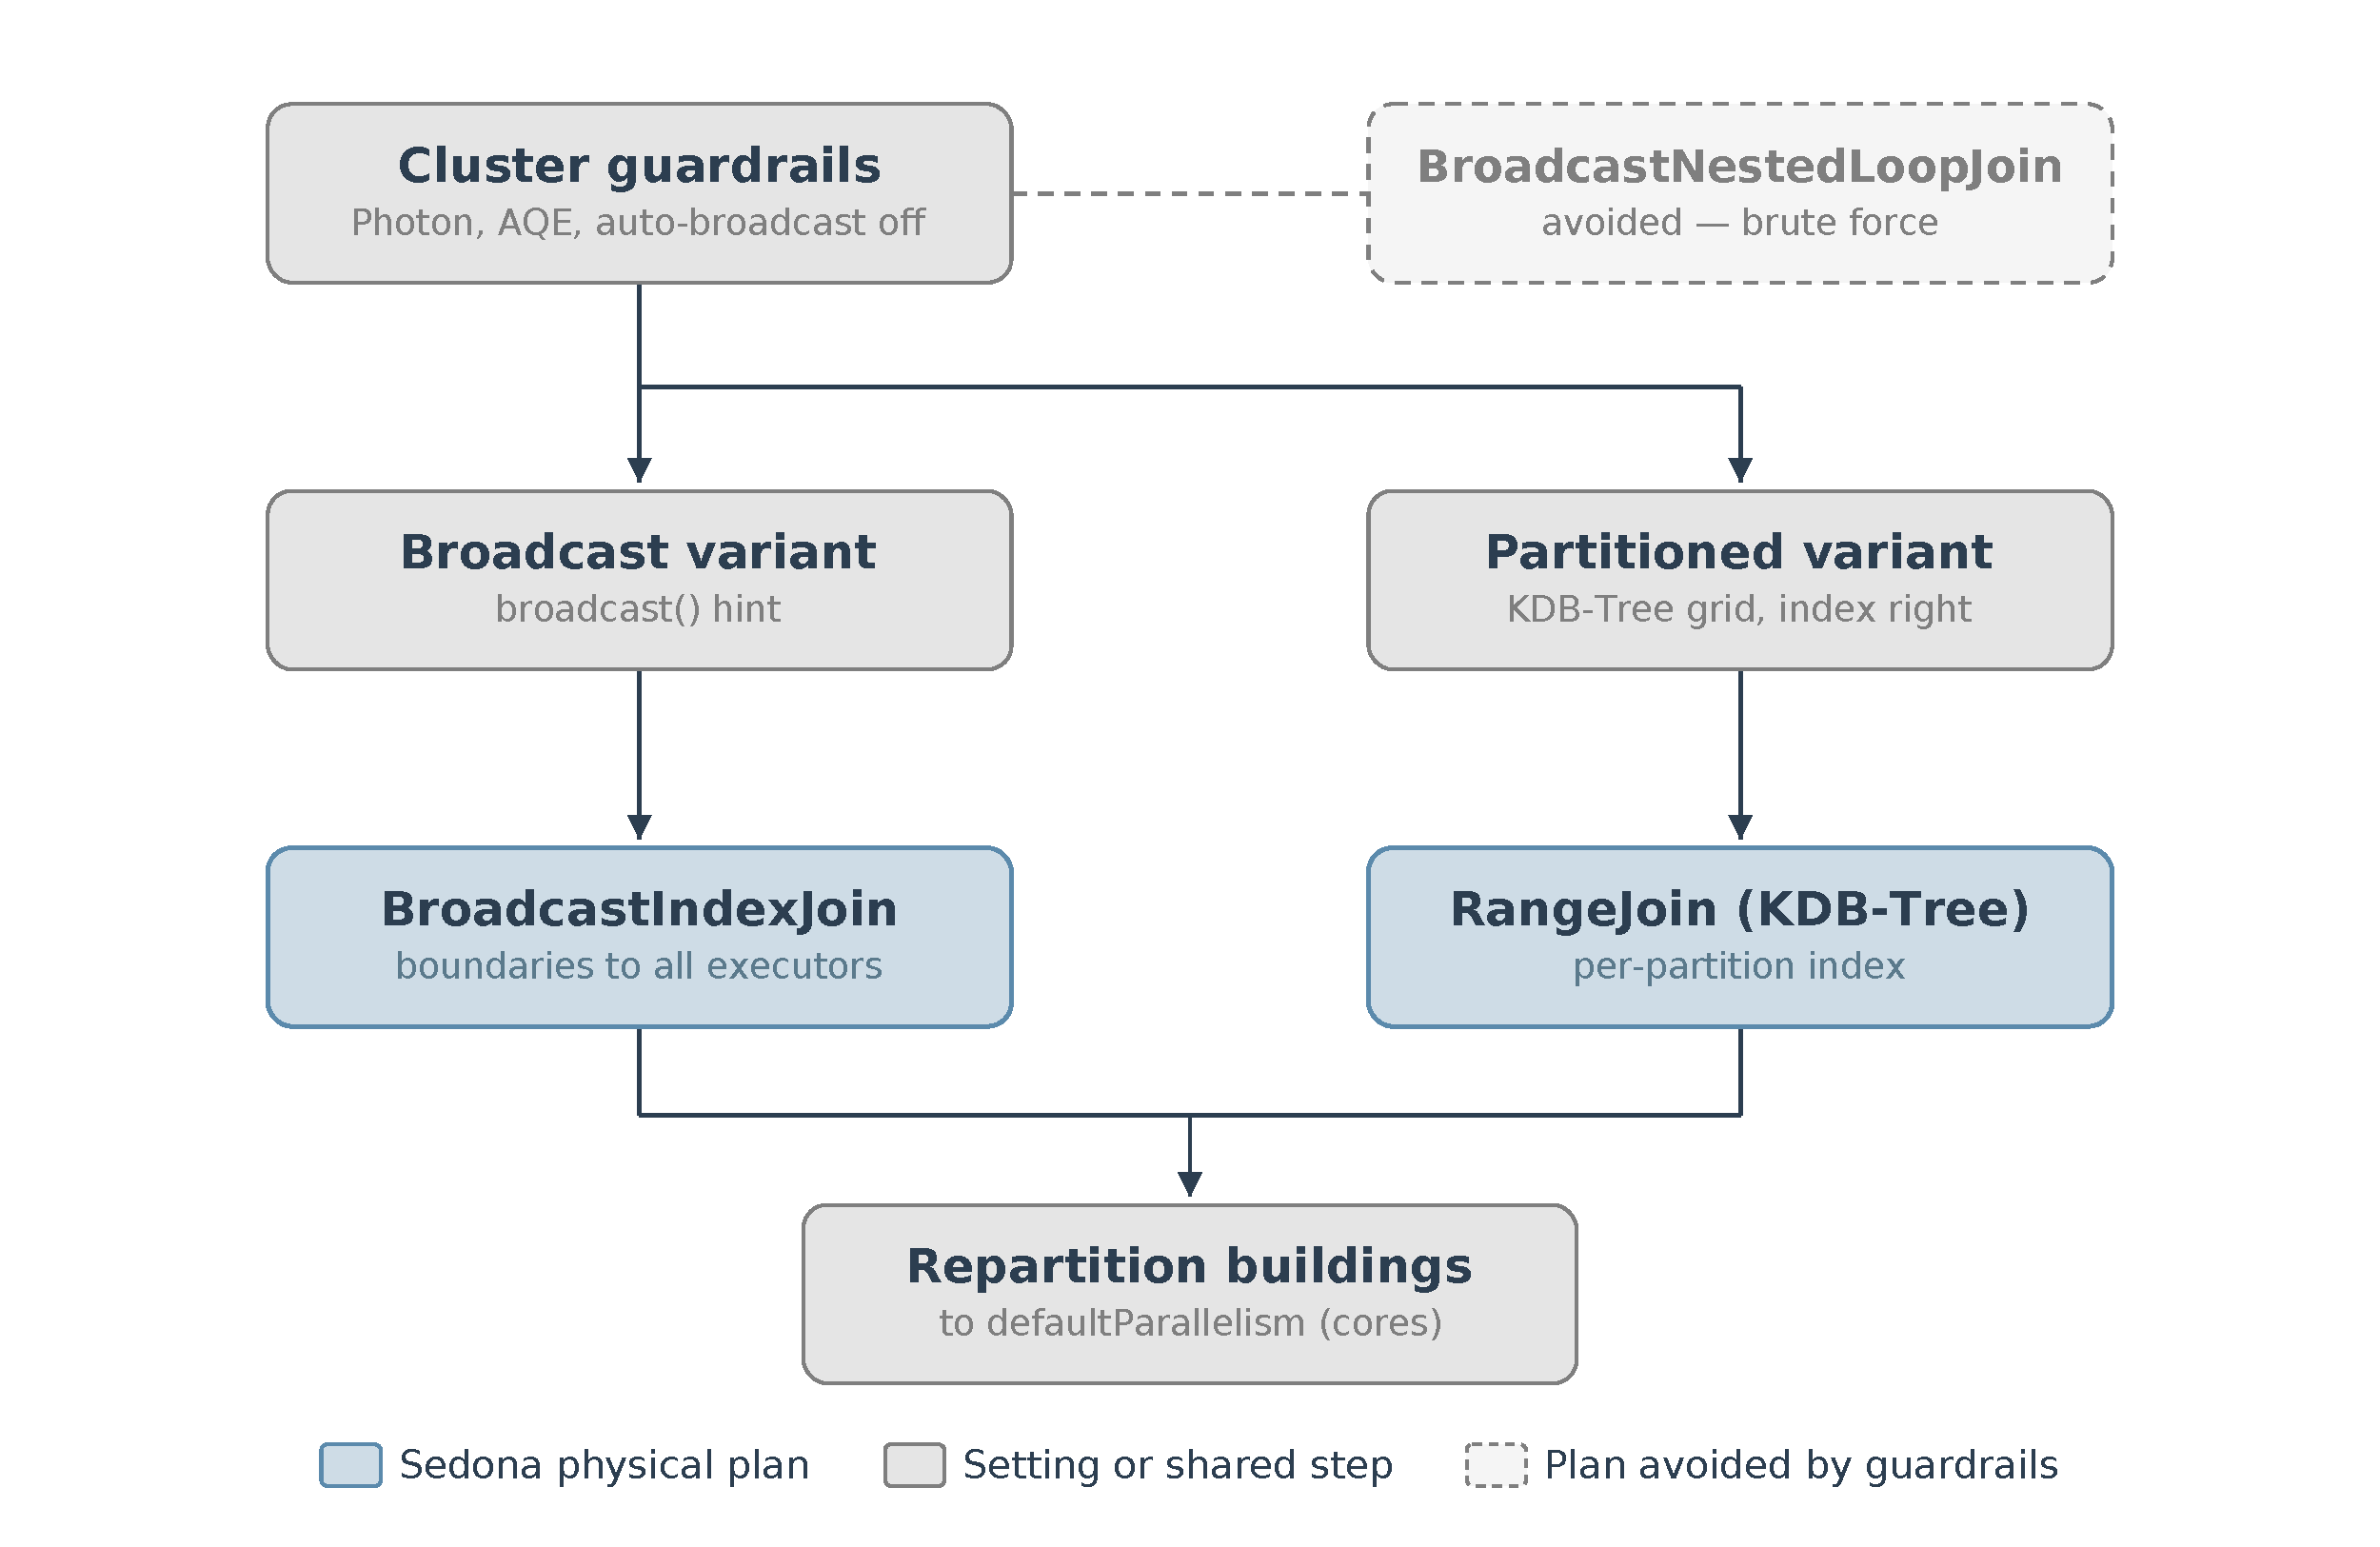
\includegraphics[width=0.8\textwidth]{Chapters/04-system-architecture-and-implementation/sub-chapters/figures/04-sedona-join-plan-control.pdf}
    \caption[Configuration controlling the Sedona spatial join plan]{Configuration controlling the Sedona spatial join plan. The shared cluster guardrails (\texttt{spark.databricks.photon.enabled=false}, \texttt{spark.sql.adaptive.enabled=false}, and \texttt{spark.sql.autoBroadcastJoinThreshold=-1}) keep Photon from forcing a BroadcastNestedLoopJoin and prevent the broadcast heuristic from pre-empting the partitioned strategy. The broadcast variant's \texttt{broadcast()} hint resolves to a BroadcastIndexJoin, while the partitioned variant's KDB-Tree settings resolve to a RangeJoin over a KDB-Tree partitioning; both repartition the buildings to the cluster's \texttt{defaultParallelism}.}
    \label{fig:sedona-join-plan-control}
\end{figure}